% %!TEX program = xelatex
\documentclass[a4paper]{oblivoir}

%%% 전처리부 (preamble)
\usepackage{intothemath}
\usepackage{fancyhdr}
\usepackage{indentfirst}
\usepackage{graphicx}
\usepackage{tcolorbox}
\usepackage[left = 2cm, right = 3cm, top = 2.5cm, bottom = 2cm, a4paper]{geometry}
\usepackage{marginnote}
\usepackage{tikz}
\usepackage{tikzpagenodes}
\usepackage{lipsum}
\usepackage{color}
\usepackage{fontspec}
\usepackage{kotex}
\usepackage{hyperref}
\hypersetup{
    colorlinks=true,
    linkcolor=blue,
    filecolor=magenta,      
    urlcolor=blue,
    pdftitle={Overleaf Example},
    pdfpagemode=FullScreen,
}
\definecolor{skyblue}{RGB}{150, 210, 250}
\definecolor{header}{RGB}{60, 120, 250}
\definecolor{subheader}{rgb}{0.19, 0.55, 0.91}

\definecolor{Axiom}{rgb}{0.0, 0.25, 0.42}
\colorlet{Definition}{blue!35!skyblue}
\definecolor{Theorem}{rgb}{0.0, 0.62, 0.42}

\setmainhangulfont[Path=FONT/]{KOPUBWORLD_BATANG_PRO_LIGHT.OTF}

%%%%%%%%%%%%%%%%% 코드 세팅 %%%%%%%%%%%%%%%%%
\definecolor{dkgreen}{rgb}{0,0.6,0}
\definecolor{mauve}{rgb}{0.58,0,0.82}
\definecolor{denim}{rgb}{0.08, 0.38, 0.74}
\definecolor{backcolour}{rgb}{0.94, 1.0, 1.0}
% \definecolor{backcolour}{rgb}{0.94, 1.0, 0.94} - 연두
% \definecolor{backcolour}{rgb}{0.91, 1.0, 1.0} - 하늘 

\lstset{frame=tb,
  language=C++,
  basicstyle=D2CODING.TTF,
  xleftmargin=15pt,
  xrightmargin=15pt,
  aboveskip=3mm,
  belowskip=3mm,
  breaklines=true, showlines=true
  showstringspaces=false,
  columns=flexible,
  basicstyle={\small\ttfamily},
  backgroundcolor=\color{backcolour},
  keepspaces=true,  
  numbers=left,       
  numbersep=7pt, 
  numberstyle=\tiny\color{black},
  keywordstyle=\color{denim},
  commentstyle=\color{dkgreen},
  stringstyle=\color{mauve},
  breaklines=true,
  breakatwhitespace=true,
  tabsize=4
}
%%%%%%%%%%%%%%%%%%%%%%%%%%%%%%%%%%%%%%%%%%%%

\begin{document}

% 1페이지

\begin{flushleft}
    {\setmainfont[Path=FONT/]{KOPUBWORLD_DOTUM_PRO_BOLD.OTF} {\textcolor{skyblue2}{{\huge\textbf{1.}}}}}
    {\setmainhangulfont[Path=FONT/]{KOPUBWORLD_DOTUM_PRO_BOLD.OTF} {\textcolor{skyblue2}{{\huge\textbf{다각형}}}}}
\end{flushleft}

\begin{flushleft}
    칠각형의 한 꼭짓점에서 그을 수 있는 대각선의 개수는 4개이며, 
    이 대각선으로 \\ 5개의 삼각형이 만들어진다.
    이때, 삼각형의 세 내각의 크기의 합은 $180^{\circ}$이므로
    칠각형의 내각의 크기의 합은 $900^{\circ}$임을 알 수 있다. 
\end{flushleft}

\begin{flushleft}
    {$(1)$ $n$각형의 대각선의 총 개수는 $\frac{n(n-3)}{2}$개이다.}
\end{flushleft}

\begin{tcolorbox}[colback = white, colframe = blue!35!skyblue, title = \textmd{이해하기}]
    $n$각형의 한 꼭짓점에서 그을 수 있는 대각선은 $(n-3)$개이므로
    $n$개의 꼭짓점에서 그을 수 있는 대각선은 $n(n-3)$개이다.
    \,그러나 한 대각선 위에는 $2$개의 꼭짓점이 있으므로 $n$각형의 대각선은
    $\frac{n(n-3)}{2}$개이다.
\end{tcolorbox}

% \marginpar{\tcbset{colback = skyblue!5!white, colframe = skyblue!99!black}
%             \begin{tcolorbox}[width = 4cm]
%                 1) 지금부터 각주를 써보도록 합시다.
%                 각주가 뭐냐고요? 아 몰라요 ㅋㅋ
%             \end{tcolorbox}}

\begin{flushleft}
    $(2)$ $n$각형의 내각의 크기의 합은 $180^{\circ} \times (n-2)$개이다.
\end{flushleft}

\begin{tcolorbox}[colback = white, colframe = blue!35!skyblue, title = \textmd{이해하기}]
    $n$각형은 $(n-2)$개의 삼각형으로 쪼개어지므로 $n$각형의 내각의 크기의 합은
    $(n-2)$개의 삼각형의 내각의 크기의 합과 같다. 이때 삼각형의 내각의 크기의 합은
    $180^{\circ}$이므로 $n$각형의 내각의 크기의 합은 $180^{\circ} \times (n-2)$이다.
\end{tcolorbox}

\begin{flushleft}
    $(3)$ $n$각형의 외각의 크기의 합은 $360^{\circ}$이다.
\end{flushleft}

% \marginpar{\tcbset{colback = skyblue!5!white, colframe = skyblue!99!black}
%             \begin{tcolorbox}[width = 4cm]
%                 2) 한 번 더 각주를 써보도록 합시다.
%                 각주가 뭐냐고요? 아 모른다구요 ㅋㅋㅋㅋㅋ
%             \end{tcolorbox}}

\begin{tcolorbox}[colback = white, colframe = blue!35!skyblue, title = \textmd{이해하기}]
    다각형의 한 꼭짓점에서의 외각과 내각의 크기의 합은 $180^{\circ}$이므로 \\ $n$각형의 모든 꼭짓점에서의
    외각과 내각의 크기의 합은  $180^{\circ} \times n$이다. \\
    즉, (외각의 크기의 합) $+$ (내각의 크기의 합) $= 180^{\circ} \times n$ \\ 
    $\therefore$ (외각의 크기의 합) $= 180^{\circ} \times n -$ (내각의 크기의 합) \\
    $= 180^{\circ} \times n - 180^{\circ} \times (n-2) = 360^{\circ}$ \\
    따라서, $n$각형의 외각의 크기의 합은 $n$의 값에 관계없이 항상 $360^{\circ}$가 된다.
\end{tcolorbox}

\begin{flushleft}
    $(4)$ 삼각형의 한 외각의 크기는 그와 이웃하지 않는 두 내각의 크기의 합과 같다.
\end{flushleft}

\begin{tcolorbox}[colback = white, colframe = blue!35!skyblue, title = \textmd{이해하기}]
    $\overline{AB} \parallel \overline{EC}$일 때, $\angle A = \angle ACE$ (엇각) $\angle B = \angle ECD$(동위각)이므로\\ 
    $\angle A + \angle B + \angle C = \angle ACE + \angle ECD + \angle BCA = 180^{\circ}$ \\
    따라서, $\angle C$의 외각 $\angle ACD$의 크기는 $\angle ACD = \angle ACE + \angle ECD = \angle A + \angle B$
    
\end{tcolorbox}
\newpage
% 2페이지

\begin{flushleft}
    {\setmainfont[Path=FONT/]{KOPUBWORLD_DOTUM_PRO_BOLD.OTF}\textcolor{skyblue2}{{\huge\textbf{2.}}}}
    {\setmainhangulfont[Path=FONT/]{KOPUBWORLD_DOTUM_PRO_BOLD.OTF}\textcolor{skyblue2}{{\huge\textbf{닮음비와 넓이 $\cdot$ 부피와 비의 관계}}}}

\end{flushleft}

\begin{flushleft}
    칠각형의 한 꼭짓점에서 그을 수 있는 대각선의 개수는 4개이며, 
    이 대각선으로 \\ 5개의 삼각형이 만들어진다.
    이때, 삼각형의 세 내각의 크기의 합은 $180^{\circ}$이므로
    칠각형의 내각의 크기의 합은 $900^{\circ}$임을 알 수 있다. 
\end{flushleft}

\begin{flushleft}
    $(1)$ $n$각형의 내각의 크기의 합은 $180^{\circ} \times (n-2)$개이다.
\end{flushleft}

\begin{tcolorbox}[colback = white, colframe = blue!35!skyblue, title = \textmd{이해하기}]
    $n$각형의 한 꼭짓점에서 그을 수 있는 대각선은 $(n-3)$개이므로
    $n$개의 꼭짓점에서 그을 수 있는 대각선은 $n(n-3)$개이다.
    \,그러나 한 대각선 위에는 $2$개의 꼭짓점이 있으므로 $n$각형의 대각선은
    $\frac{n(n-3)}{2}$개이다.
\end{tcolorbox}

\begin{flushleft}
    $(2)$ $n$각형의 내각의 크기의 합은 $180^{\circ} \times (n-2)$개이다.
\end{flushleft}



\begin{flushleft}
    {\setmainfont[Path=FONT/]{KOPUBWORLD_DOTUM_PRO_BOLD.OTF}\textcolor{skyblue2}{{\huge\textbf{3.}}}}
    {\setmainhangulfont[Path=FONT/]{KOPUBWORLD_DOTUM_PRO_BOLD.OTF}\textcolor{skyblue2}{{\huge\textbf{평행선과 넓이}}}}
\end{flushleft}

\begin{flushleft}
    $(3)$ 삼각형의 한 외각의 크기는 그와 이웃하지 않는 두 내각의 크기의 합과 같다.
\end{flushleft}

\begin{tcolorbox}[colback = white, colframe = blue!35!skyblue, title = \textmd{이해하기}]
    $\overline{AB} \parallel \overline{EC}$일 때, $\angle A = \angle ACE$ (엇각) $\angle B = \angle ECD$(동위각)이므로\\ 
    $\angle A + \angle B + \angle C = \angle ACE + \angle ECD + \angle BCA = 180^{\circ}$ \\
    따라서, $\angle C$의 외각 $\angle ACD$의 크기는 $\angle ACD = \angle ACE + \angle ECD = \angle A + \angle B$
\end{tcolorbox}


\begin{flushleft}
    {\setmainfont[Path=FONT/]{KOPUBWORLD_DOTUM_PRO_BOLD.OTF}\textcolor{skyblue2}{{\huge\textbf{4.}}}}
    {\setmainhangulfont[Path=FONT/]{KOPUBWORLD_DOTUM_PRO_BOLD.OTF}\textcolor{skyblue2}{{\huge\textbf{프로그래밍 실습}}}}
\end{flushleft}

\begin{flushleft}
    $(4)$ JAVA 언어로 Hello World를 출력해보도록 하겠습니다.
\end{flushleft}

\begin{lstlisting}
// HelloWorld.cpp
#include <iostream>

using namespace std;

int main() {
    cout << "Hello World!!" << endl;
    return 0;
}
\end{lstlisting}
\newpage
% 3페이지


\section{Introduction}
Your introduction goes here! Simply start writing your document and use the Recompile button to view the updated PDF preview. Examples of commonly used commands and features are listed below, to help you get started.

Once you're familiar with the editor, you can find various project settings in the Overleaf menu, accessed via the button in the very top left of the editor. To view tutorials, user guides, and further documentation, please visit our 

\subsection{How to create Sections and Subsections}

Simply use the section and subsection commands, as in this example document! With Overleaf, all the formatting and numbering is handled automatically according to the template you've chosen. If you're using Rich Text mode, you can also create new section and subsections via the buttons in the editor toolbar.

\subsection{How to write Mathematics}

\LaTeX{} is great at typesetting mathematics. Let $X_1, X_2, \ldots, X_n$ be a sequence of independent and identically distributed random variables with $\text{E}[X_i] = \mu$ and $\text{Var}[X_i] = \sigma^2 < \infty$, and let
\[S_n = \frac{X_1 + X_2 + \cdots + X_n}{n}
      = \frac{1}{n}\sum_{i}^{n} X_i\]
denote their mean. Then as $n$ approaches infinity, the random variables $\sqrt{n}(S_n - \mu)$ converge in distribution to a normal $\mathcal{N}(0, \sigma^2)$.

\subsection{How to include Figures}

First you have to upload the image file from your computer using the upload link in the file-tree menu. Then use the includegraphics command to include it in your document. Use the figure environment and the caption command to add a number and a caption to your figure. See the code for Figure \ref{fig:Jesus} in this section for an example.

Note that your figure will automatically be placed in the most appropriate place for it, given the surrounding text and taking into account other figures or tables that may be close by. You can find out more about adding images to your documents in this help article on \href{https://www.overleaf.com/learn/how-to/Including_images_on_Overleaf}{including images on Overleaf}.

\begin{figure} [h]
\centering
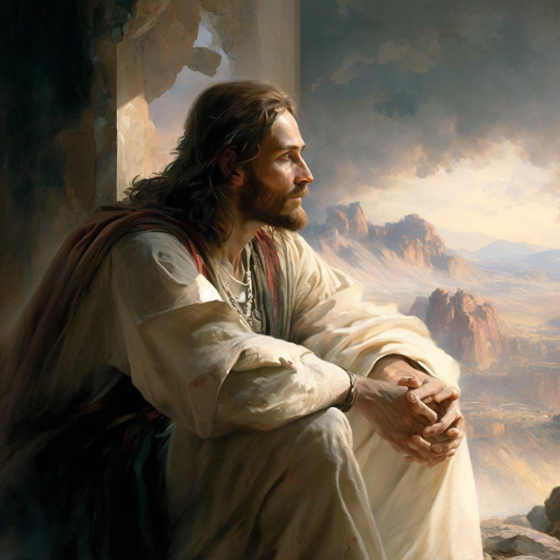
\includegraphics[width=0.3\textwidth]{Jesus.png}
\caption{\label{fig:Jesus}Jesus was uploaded via the file-tree menu.}
\end{figure}

\subsection{How to add Tables}

Use the table and tabular environments for basic tables --- see Table~\ref{tab:widgets}, for example. For more information, please see this help article on \href{https://www.overleaf.com/learn/latex/tables}{tables}. 

\begin{table}
\centering
\begin{tabular}{l|r}
Item & Quantity \\\hline
Widgets & 42 \\
Gadgets & 13
\end{tabular}
\caption{\label{tab:widgets}An example table.}
\end{table}
\newpage

\end{document}

